\section{Decision Trees}

    Il $\textbf{Decision Tree Learning}$ è un approccio di apprendimento supervisionato che utilizza un albero decisionale di classificazione o regressione che verrà utilizzato come modello predittivo per trarre conclusioni su un insieme di osservazioni.
    \\[1\baselineskip]
    I modelli ad albero in cui la variabile target può assumere un insieme discreto di valori sono chiamati $\textit{alberi di classificazione}$; in queste strutture ad albero, le foglie rappresentano etichette di classe e i rami rappresentano congiunzioni di caratteristiche che portano a quelle etichette di classe.
    Gli alberi decisionali in cui la variabile target può assumere valori continui (tipicamente numeri reali) sono chiamati $\textit{alberi di regressione}$.
    
    \begin{figure}[h]
        \caption{Esempio di Decision Tree}
        \centering
        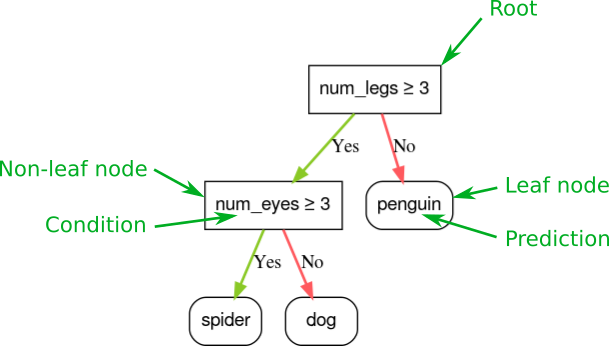
\includegraphics[width = 8cm, height = 4.2cm]{DecisionTree.png}
    \end{figure}

    \subsection{Condizioni Verticali vs Oblique}
        Una condizione verticale (o anche detta "allineata agli assi", "split verticale") coinvolge una sola feature mentre una condizione obliqua coinvolge molteplici features.
        Per esempio, $\textit{num\_legs} \geq 2$ è una condizione verticale mentre $\textit{num\_legs} \geq \textit{num\_eyes}$ è una condizione obliqua.
        \\[1\baselineskip]
        Spesso i Decision Trees sono allenati su condizioni verticali. Tuttavia, lo splitting obliquo è molto più potente perché può esprimere pattern più complessi e può produrre risultati migliori, ad un elevato costo computazionale per il train e l'inferenza.

        \begin{figure}[h]
            \caption{Esempio di Splitting}
            \centering
            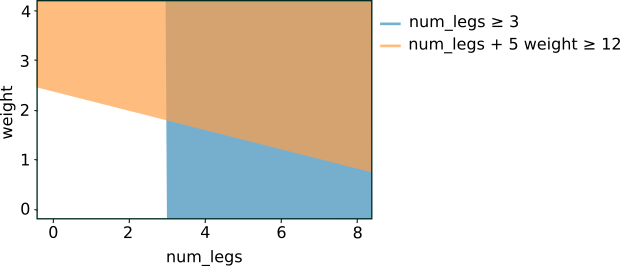
\includegraphics[width = 10cm]{decisiontrees-conditions.png}
        \end{figure}

    \clearpage

    \subsection{Condizioni Binarie vs Non-Binarie}
        Condizioni con due possibili risultati (ad esempio, vero o falso) sono chiamate condizioni binarie.
        Alberi decisionali contenenti solo condizioni binari sono chiamati $\textit{Binary Decision Trees}$.
        \\[1\baselineskip]
        Le condizioni non binarie hanno più di due possibili esiti, dunque hanno un potere discriminante maggiore rispetto a quelle binarie.
        Gli alberi che contengono decisioni una o più condizioni non binarie sono chiamati $\textit{Non-Binary Decision Trees}$.
        \\[1\baselineskip]
        $\textbf{Attenzione}$: Le condizioni non binarie hanno maggiore probabilità di overfit
        
    \subsection{Elenco delle Condizioni più Usate}
        Giusto per essere completi, ecco un elenco dei tipi condizioni che vengono comunemente utilizzate:

        \begin{figure}[h]
            \centering
            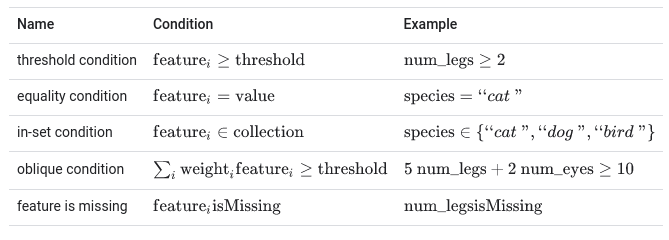
\includegraphics[width = 8.5cm]{conditions-types.png}
        \end{figure}
    
    \clearpage

    \subsection{Costruire un Decision Tree}
        La costruzione del migliore albero decisionale è un problema NP-Hard, dunque viene generalmente utilizzata un'euristica per costruire un albero ottimale.
        La maggior parte degli algoritmi utilizzati per allenare gli alberi decisionali funziona con una strategia greedy in stile $\textit{divide et impera}$: l'algoritmo inizia creando un singolo nodo (la radice) e cresce ricorsivamente, e in maniera greedy, l'albero decisionale.
        Ad ogni nodo, tutte le possibili condizioni vengono valutate e viene assegnato a loro un punteggio; l'algoritmo seleziona la condizione "migliore", ovvero la condizione con il punteggio più alto.\\
        Dopodiché viene eseguito lo split sulla base della condizione precedentemente scelta.
        \\[1\baselineskip]
        L'algoritmo, quindi, ripete ricorsivamente e indipendentemente su tutti i nodi figli, valutando condizioni che non sono ancora state scelte come condizioni di split.
        Quando non vengono trovate condizioni soddisfacenti, il nodo diventa una foglia.
        La predizione nella foglia è scelta come il valore dell'etichetta più significativo.

        \clearpage

        \begin{figure}[h]
            \caption{Esempio di Creazione}
            \centering
            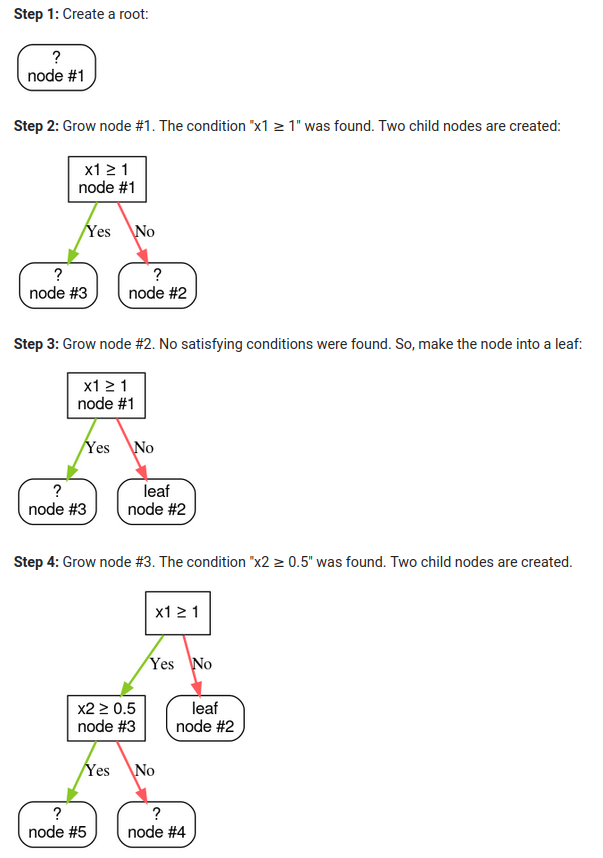
\includegraphics[width = 10cm, height = 12cm]{building-tree-steps.png}
        \end{figure}

        \clearpage

    \subsection{Misura dell'Impurità del Singolo Nodo}
    L'impurità di un nodo misura quanto sono differenti le etichette delle classi per le istanze di dati appartenenti a un nodo comune.
    \\[1\baselineskip]
    Alcune misure che possono essere utilizzate per misurare l'impurità di un certo nodo $t$ sono:

    \begin{itemize}
        \item $\textbf{Entropy}$: $-\sum_{i = 0}^{m-1}{p_{i}(t) \cdot \log_{2}{(p_{i}(t))}}$
            \\[0.5\baselineskip]
            - Massimo: $\log m$, dove $m$ è il numero di classi, quando i records sono equamente distribuiti su tutte le classi, implica poca informazione;
            \\[0.5\baselineskip]
            - Minimo: 0.0 quando tutti i recordi appartengono a una sola classe, implica maggiore informazione (assumiamo che $0 \cdot \log(0) = 0$) (\textbf{"Foglia Pura"}).
            \\
        \item $\textbf{Gini Index}$: $1 - \sum_{i = 0}^{m-1}{p_{i}(t)^{2}}$
            \\[0.5\baselineskip]
            - Massimo: $(1 - \frac{1}{m})$ quando i records sono equamente distribuiti su tutte le classi, implica poca informazione;
            \\[0.5\baselineskip]
            - Minimo: 0.0 quando tutti i records appartengono a una sola classe, implica maggiore informazione.
            \\
        \item $\textbf{Classification Error}$: $1 - \max{[p_{i}(t)]},\ \forall{i}$
            \\[0.5\baselineskip]
            - Massimo: $(1 - \frac{1}{m})$, dove $m$ è il numero di classi, quando i records sono equamente distribuiti su tutte le classi, implica poca informazione;
            \\[0.5\baselineskip]
            - Minimo: 0.0 quando tutti i records appartengono a una classe, implica maggiore informazione.
            \\
        \item $\textbf{Gain Ratio}$: $\frac{\Delta_{\textrm{info}}}{\textrm{SplitInfo}({\cal D})}$ (vedi sotto per $\Delta_{\textrm{info}}$)
            \\[0.5\baselineskip]
            - dove $\textrm{SplitInfo}({\cal D}) = -\sum_{i=0}^{k} {\left[\frac{N(v_{i})}{N} \cdot \log_{2}(\frac{N(v_{i})}{N})\right]}$ con $N(v_{i}) =$ numero di istanze di
                training associate al nodo $v_{i}$ e $N =$ numero di istante di training;
            \\[0.5\baselineskip]
            - Gain Ratio normalizza l'Information Gain per lo SplitInfo di uno split k-ario.
                Per Decision Trees k-ari (invece che binari), l'Information Gain favorisce gli splits con molte piccole partizioni (è più probabile che siano pure);
            \\[0.5\baselineskip]
            - È usato per compensare attributi che producono un gran numero di nodi figlio.
            \\
    \end{itemize}

    dove $p_{i}(t)$ è la frequenza delle istanze di training che appartengono alla classe $i$ al nodo $t$ e $m$ è il numero totale di classi.

    \begin{figure}[h]
        \caption{Cattivo Split vs Buono Split}
        \centering
        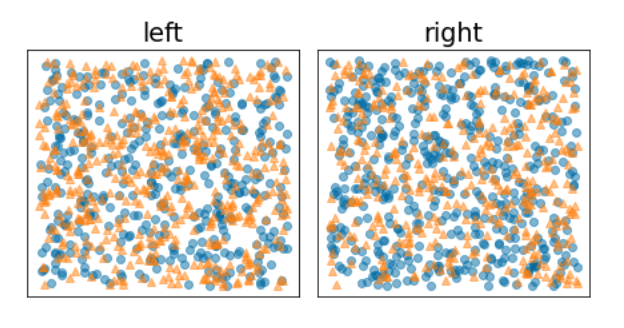
\includegraphics[width = 10cm, height = 6cm]{bad-splitting.png}
        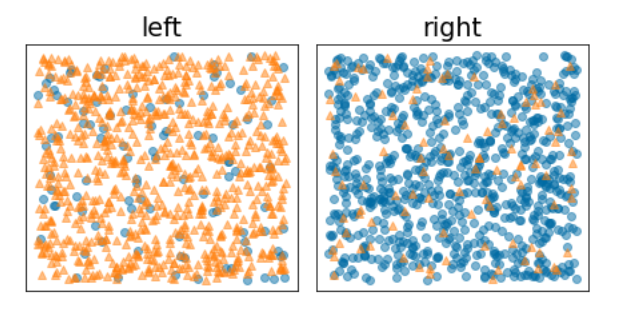
\includegraphics[width = 10cm, height = 6cm]{good-splitting.png}
    \end{figure}

    \clearpage

    \subsection{Impurità Collettiva dei Nodi Figlio}
        Possiamo calcolare l'impurità dei nodi figlio come:
            $$ I(children) = \sum_{i=0}^{k} {\left[\frac{N(v_{i})}{N} \cdot I(v_{i})\right]} $$
        dove:
        \begin{itemize}
            \item $k$ è il numero di nodi figlio;
            \item $N$ è il numero delle istanze di training;
            \item $N(v_{i})$ è il numero di istanze di training associate con il nodo $v_{i}$;
            \item $I(v_{i})$ è l'impurità del nodo $v_{i}$ calcolata con le formule di errore viste prima.
        \end{itemize}

        $\textbf{Esempio:}$ Consideriamo i candidati (a) e (b) per il test della condizione del problema di classificazione dei mutuatari, mostrati nella figura sottostante.
        \begin{figure}[h]
            \centering
            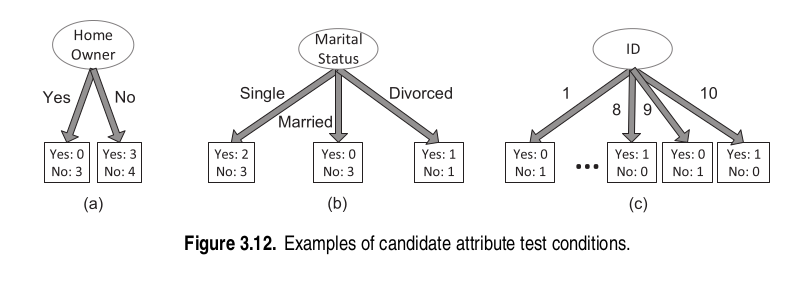
\includegraphics[width = 10cm, height = 3.1cm]{impurity-example.png}
        \end{figure}

        Calcoliamo la $\textbf{Weighted Entropy}$ di Home Owner come segue:
            $$ I(\textrm{Home Owner = Yes}) = - \frac{0}{3} \cdot \log_{2}(\frac{0}{3}) - \frac{3}{3} \cdot \log_{2}(\frac{3}{3}) = 0 $$
            $$ I(\textrm{Home Owner = No}) = - \frac{3}{7} \cdot \log_{2}(\frac{3}{7}) - \frac{4}{7} \cdot \log_{2}(\frac{4}{7}) = 0.985 $$
            $$ I(\textrm{Home Owner}) = \frac{3}{10} \cdot 0 + \frac{7}{10} \cdot 0.985 = 0.690 $$
        \\[1\baselineskip]
        Ora la calcoliamo anche per Marital Status:
            $$ I(\textrm{Marital Status = Single}) = - \frac{2}{5} \cdot \log_{2}(\frac{2}{5}) - \frac{3}{5} \cdot \log_{2}(\frac{3}{5}) = 0.971 $$
            $$ I(\textrm{Marital Status = Married}) = - \frac{0}{3} \cdot \log_{2}(\frac{0}{3}) - \frac{3}{3} \cdot \log_{2}(\frac{3}{3}) = 0 $$
            $$ I(\textrm{Marital Status = Divorced}) = - \frac{1}{2} \cdot \log_{2}(\frac{1}{2}) - \frac{1}{2} \cdot \log_{2}(\frac{1}{2}) = 1.000 $$
            $$ I(\textrm{Marital Status}) = \frac{5}{10} \cdot 0.971 + \frac{3}{10} \cdot 0 + \frac{2}{10} \cdot 1.0 = 0.686 $$
            \\[1\baselineskip]
        Come possiamo vedere, l'impurità di Marital Status è leggermente più alta rispetto a Home Owner.

        \clearpage

        \subsection{Trovare la migliore condizione per il test degli attributi}
            Per determinare la bontà di una condizione di test, dobbiamo confrontare il grado di impurità del nodo genitore (prima della divisione) con il grado pesato di impurità dei nodi figli (dopo la divisione).
            \\
            Maggiore è la loro differenza, migliore è la condizione del test. Questa differenza, $\Delta$, definita anche come il guadagno ($\textbf{Gain}$) in purezza di una condizione di test, può essere definita come segue:
                $$ \Delta = I(\textrm{parent}) - I(\textrm{children}) $$

            Maggiore è il guadagno, più pure sono le classi nei nodi figli rispetto al nodo genitore. Il criterio di suddivisione nell'algoritmo di Decision Tree seleziona la condizione di test che mostra il guadagno massimo.
            \\[1\baselineskip]
            Infine, quando l'entropia è usata come misura di impurità, la differenza di entropia tra genitore e figli è comunemente nota come $\textbf{Information Gain}$, $\Delta_{\text{info}}$.

            \begin{figure}[h]
                \centering
                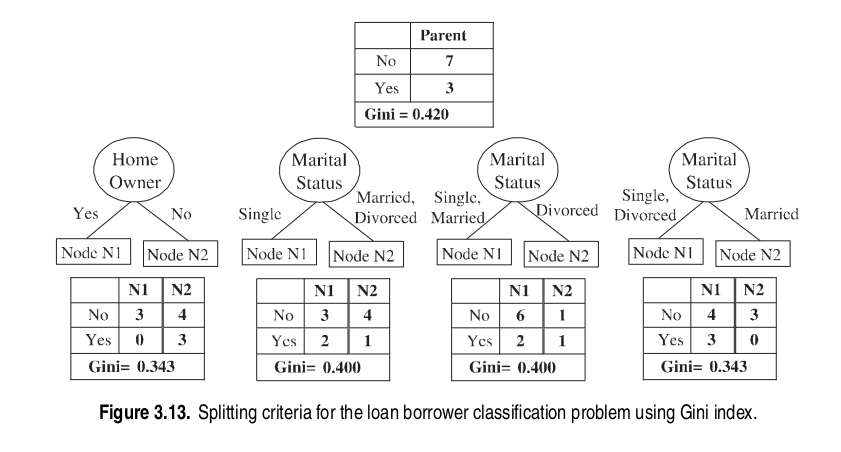
\includegraphics[width = 10cm, height = 6.5cm]{best-attribute-example.png}
            \end{figure}

            \clearpage
